\section{Results}
\label{sec:results}

We report results in four parts that follow the argument of the paper. We first establish a \emph{faithful replication} of the original pipeline under image-level sampling, and isolate the single pooling choice that controls its accuracy (Sec.~\ref{subsec:replication}). We then give the \emph{best estimator under each of the two sampling protocols}, an Optuna-tuned stacked ensemble, and place it against the EMBC~2019 figures (Sec.~\ref{subsec:dual}). We next ask whether a stronger backbone is the right lever, through an \emph{architecture bake-off} under patient-level cross-validation (Sec.~\ref{subsec:bakeoff}). Finally we trace the \emph{methods progression} that yields the patient-level estimator (Sec.~\ref{subsec:progression}). Throughout, $\theta$ denotes the Doppler beam-to-vessel angle, operationalized here as the magnitude of applied image rotation (Sec.~\ref{sec:methods}). Mean absolute error (MAE) and root-mean-square error (RMSE) are reported in degrees, mean absolute percentage error (MAPE) as a percentage, and the coefficient of determination $R^2$ is unitless. All runs use seed~42 under Keras~3 / JAX.

The two sampling protocols are both legitimate and answer different questions. \emph{Image-level sampling} draws the train/test partition over the rotation-augmented corpus and measures accuracy across the population of orientations and imaging conditions the augmentation spans; this is the protocol of the original study. \emph{Patient-level sampling} holds out whole volunteers via \texttt{GroupKFold} and measures generalization to a previously unseen patient. We report and tune both.

\subsection{Faithful replication under image-level sampling}
\label{subsec:replication}

We reproduce the EMBC~2019 pipeline~\citep{Patil2019} under image-level sampling. The 84 longitudinal common-carotid B-mode images are rotation-augmented over $[-60,+60]\si{\degree}$ in \SI{5}{\degree} steps, giving \num{25} oriented views each and $\approx\!2{,}100$ labelled examples, and partitioned into train and test at the image level. Table~\ref{tab:replication} pairs frozen ImageNet backbones~\citep{Deng2009} (\texttt{include\_top=False}, no fine-tuning) with the orientation-preserving grid-pooling head.

The pooling operator is the design choice that governs accuracy here. Global average pooling collapses the convolutional feature map over all spatial positions and is therefore approximately rotation-invariant. That is the wrong inductive bias when the regression target is itself an orientation, because $\theta$ is exactly the quantity a rotation-invariant summary discards. A grid-pooling head instead average-pools the feature map to a small $G\times G$ grid and then flattens, preserving the coarse spatial arrangement of activations and retaining the orientation signal the target depends on.

This change alone roughly halves the frozen DenseNet201~\citep{Huang2017} error. Under image-level five-fold cross-validation it falls from \SI{10.85}{\percent} MAPE with a global-average-pooling head to \SI{4.58}{\percent} with grid pooling. On the original single augmented split (Table~\ref{tab:replication}) the grid-pooling model reaches \SI{5.84}{\percent} MAPE (\SI{3.77}{\degree} MAE, \SI{4.75}{\degree} RMSE, $R^2=0.982$). With this head, DenseNet201 is the strongest backbone by a wide margin, recovering the single-digit-degree error band of the original report under its stated protocol and with no fine-tuning. The other backbones trail well behind under the identical head: InceptionV3~\citep{Szegedy2016} at \SI{11.70}{\percent}, Xception~\citep{Chollet2017} at \SI{12.00}{\percent}, ResNet50~\citep{He2016} at \SI{12.75}{\percent}, and VGG19~\citep{Simonyan2015} at \SI{18.01}{\percent}. This is consistent with DenseNet's dense feature reuse suiting a fine-grained orientation task.

One difference from the original report is substantive. Patil and Anand found \emph{VGG19} to be their single best backbone (\SI{2.87}{\degree} MAE), whereas under our shared grid-pooling head and fixed training budget DenseNet201 leads and VGG19 trails the field. We therefore reproduce the original error \emph{regime}, a frozen backbone reaching single-digit-degree error, but not its per-model ranking. The most likely cause is methodological. To keep the comparison controlled we hold the pooling operator, head architecture, and training budget identical across all five backbones, whereas the original tuned these per model. A configuration that suits VGG19's coarse, large-stride feature map need not be the one that suits DenseNet201's dense maps, so a single shared head can reshuffle the ranking even when the attainable accuracy is preserved. Figure~\ref{fig:pred_vs_actual} shows the per-backbone predicted-versus-actual fit, and Fig.~\ref{fig:error_vs_angle} the absolute error across the observed-angle range.

% AUTO-GENERATED by scripts/gen_paper_tables.py from results/ — DO NOT EDIT.
% Re-run: pixi run python scripts/gen_paper_tables.py
\begin{table}[htbp]
  \centering
  \caption{Faithful replication under image-level sampling (the original augmented-corpus protocol): frozen ImageNet backbones with the orientation-preserving grid-pooling head. The best configuration (DenseNet201) reaches \SI{5.84}{\percent} MAPE, reproducing Table~I of the EMBC 2019 paper.}
  \label{tab:replication}
  \begin{tabular}{llrrrrr}
    \toprule
    Backbone & Pooling & $N_{\mathrm{test}}$ & MAE (\degr) & RMSE (\degr) & MAPE (\%) & $R^2$ \\
    \midrule
    DenseNet201 & grid3 & 420 & 3.77 & 4.75 & 5.84 & 0.982 \\
    InceptionV3 & grid2 & 420 & 8.36 & 10.44 & 11.70 & 0.911 \\
    Xception & grid2 & 420 & 7.91 & 11.20 & 12.00 & 0.898 \\
    ResNet50 & grid2 & 420 & 8.97 & 11.62 & 12.75 & 0.890 \\
    VGG19 & grid2 & 420 & 11.67 & 17.77 & 18.01 & 0.743 \\
    \bottomrule
  \end{tabular}
\end{table}


\begin{figure}[htbp]
  \centering
  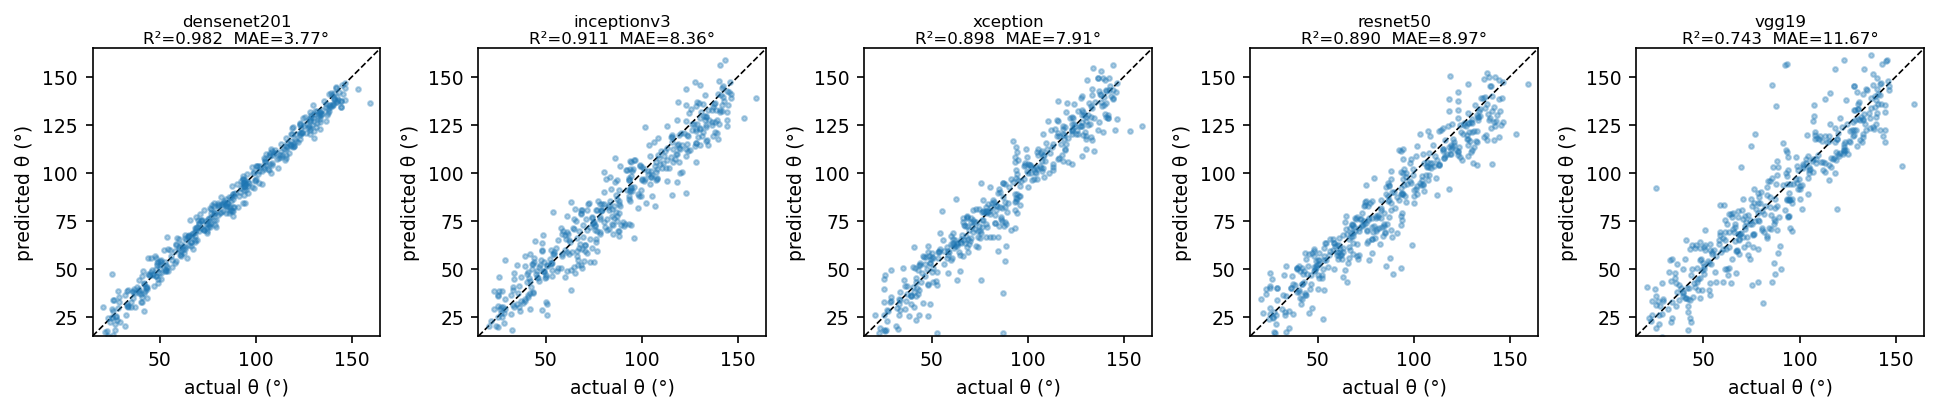
\includegraphics[width=0.92\linewidth]{figures/figure4_pred_vs_actual.png}
  \caption{Predicted versus actual Doppler angle for each frozen backbone with the grid-pooling head, under image-level sampling. Points on the diagonal are exact predictions; DenseNet201 tracks the identity line across the full angle range, while the weaker backbones scatter more widely.}
  \label{fig:pred_vs_actual}
\end{figure}

\begin{figure}[htbp]
  \centering
  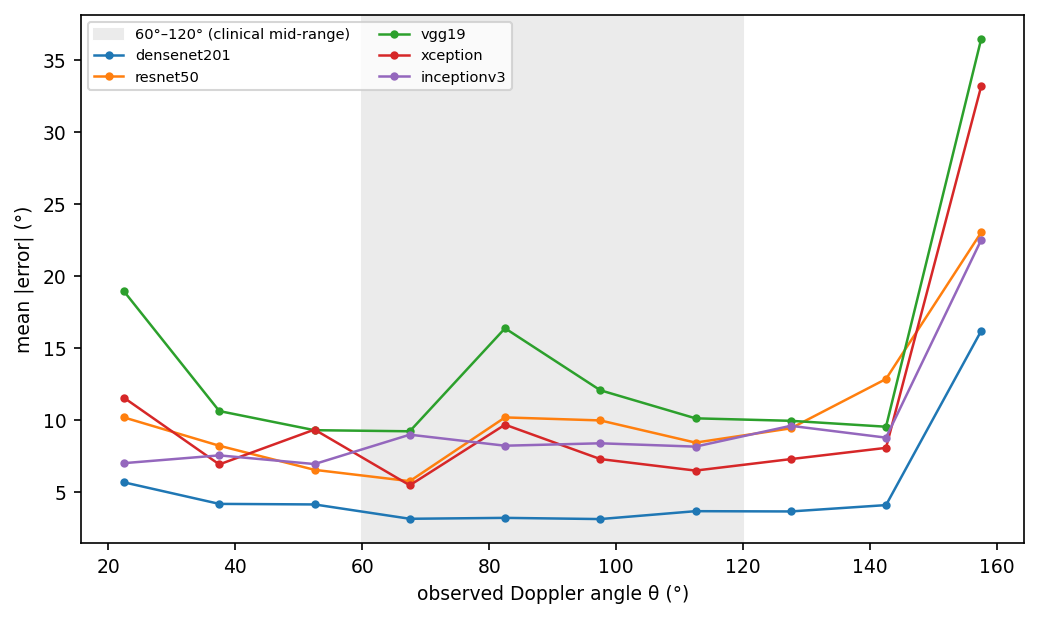
\includegraphics[width=0.7\linewidth]{figures/figure5_error_vs_angle.png}
  \caption{Mean absolute error as a function of the observed Doppler angle. For the best model (DenseNet201) the error is low and roughly flat across the mid-range and rises sharply only at the most oblique observed angle ($\sim$\SI{158}{\degree}); the weaker backbones carry larger and less stable error, with a local rise near \SI{82}{\degree}. The shaded band marks the clinically common $60$--$120\si{\degree}$ range.}
  \label{fig:error_vs_angle}
\end{figure}

\subsection{Best estimator under each sampling protocol}
\label{subsec:dual}

Table~\ref{tab:dual_protocol} reports the Optuna-tuned estimator under both sampling protocols, each tuned to its own best configuration. The head and optimizer hyperparameters (head depth and width, dropout, $L_2$ penalty, BatchNorm placement, learning rate, batch size, and early-stopping patience) are searched with the Tree-structured Parzen Estimator~\citep{Bergstra2011} as implemented in Optuna~\citep{Akiba2019}, scored by five-fold cross-validation on cached frozen features. The backbone extraction is run once per network and the cached features serve both protocols, so the two halves of the table are like-for-like up to the sampling level. Per-backbone rows are five-fold cross-validated tuned heads; ensemble rows are out-of-fold (OOF) predictions over the five tuned fold models. The two row types are thus different estimators of the same quantity, a point we return to below. Optimization uses Adam~\citep{Kingma2015} with a base learning rate of \num{1e-4} and an MSE objective; CLAHE~\citep{Zuiderveld1994} contrast normalization is applied to the inputs.

The single best backbone is DenseNet201, which reaches \SI{4.03}{\percent} MAPE (\SI{3.00}{\degree} MAE, $R^2=0.988$) under image-level sampling and \SI{10.80}{\percent} MAPE (\SI{8.62}{\degree} MAE, $R^2=0.886$) under patient-level five-fold cross-validation. Tuning the head moves DenseNet201 from the frozen \SI{4.58}{\percent} to \SI{4.03}{\percent} at image level and from \SI{12.59}{\percent} to \SI{10.80}{\percent} at patient level (frozen and tuned both five-fold CV). These shifts are small relative to the per-fold standard deviations (Table~\ref{tab:dual_protocol}), so we read tuning as a consistent but modest refinement rather than a step change. The per-backbone ordering by MAE is stable across both protocols (DenseNet201 $\geq$ ResNet50 $\geq$ VGG19 $\geq$ InceptionV3 $\approx$ Xception), so the choice of backbone is largely insensitive to the evaluation lens. Under patient-level MAPE, VGG19 at \SI{14.97}{\percent} and InceptionV3 at \SI{14.66}{\percent} sit within \SI{0.3}{} percentage points and exchange ranks.

Ensembling the five tuned backbones improves both columns. A plain OOF mean of the five members reaches \SI{3.03}{\percent} MAPE (\SI{2.09}{\degree} MAE, $R^2=0.994$) under image-level sampling and \SI{9.89}{\percent} MAPE (\SI{6.89}{\degree} MAE, $R^2=0.932$) under patient-level sampling. A stacked combiner~\citep{Wolpert1992} fitted over the OOF predictions sharpens both further, to \textbf{\SI{2.79}{\percent} MAPE (\SI{1.96}{\degree} MAE, $R^2=0.995$)} under image-level sampling and \textbf{\SI{8.53}{\percent} MAPE (\SI{5.93}{\degree} MAE, $R^2=0.952$)} under patient-level sampling. This is the first patient-level result in our progression to fall below \SI{10}{\percent} MAPE.

The size of this gain depends on how the single-model baseline is aggregated, and the like-for-like comparison is the fair one. Aggregating the single tuned DenseNet201 the same pooled-OOF way reaches \SI{7.80}{\degree} MAE / \SI{10.14}{\percent} MAPE at patient level, against its \SI{8.62}{\degree} per-fold mean in Table~\ref{tab:dual_protocol}. On the matched pooled-OOF basis the stacked ensemble improves the single best model by about \SI{1.9}{\degree} MAE. The larger apparent gap (\SI{8.62}{\degree} to \SI{5.93}{\degree}) partly reflects the per-fold-mean versus pooled-OOF aggregation, not ensembling alone, so we quote the matched figure as the ensembling gain. That the plain mean is already competitive follows from tuning: per-member calibration is good enough that a simple average works, whereas averaging the untuned heads, whose error scales differ, was far less effective.

% AUTO-GENERATED by scripts/gen_paper_tables.py from results/ — DO NOT EDIT.
% Re-run: pixi run python scripts/gen_paper_tables.py
\begin{table}[htbp]
  \centering
  \caption{Doppler-angle estimation under two sampling protocols, each Optuna-tuned to its own best configuration. \emph{Image-level sampling} draws the train/test partition over the rotation-augmented image corpus (the standard synthetic-data protocol of the original study); \emph{patient-level sampling} holds out whole volunteers, a stricter cross-subject generalization test. Per-backbone rows are patient/image five-fold cross-validated tuned heads (means; per-fold MAPE std is \SIrange{0.1}{0.7}{\percent} for image-level and \SIrange{2.6}{4.4}{\percent} for the higher-variance patient-level folds); ensemble rows are pooled out-of-fold over the five tuned models. Note the aggregation differs: member rows are per-fold means, ensemble rows are pooled OOF (the single tuned DenseNet201 aggregated pooled-OOF is \SI{7.80}{\degree} MAE patient-level, the like-for-like predecessor of the ensemble rows). Both columns are recomputed from \texttt{results/} by \texttt{scripts/gen\_paper\_tables.py}.}
  \label{tab:dual_protocol}
  \begin{tabular}{lrrrrrr}
    \toprule
    & \multicolumn{3}{c}{Image-level sampling} & \multicolumn{3}{c}{Patient-level sampling} \\
    \cmidrule(lr){2-4}\cmidrule(lr){5-7}
    Model (Optuna-tuned) & MAE (\degr) & MAPE (\%) & $R^2$ & MAE (\degr) & MAPE (\%) & $R^2$ \\
    \midrule
    DenseNet201 & 3.00 & 4.03 & 0.988 & 8.62 & 10.80 & 0.886 \\
    ResNet50 & 3.64 & 4.84 & 0.981 & 9.79 & 13.30 & 0.842 \\
    VGG19 & 4.22 & 5.79 & 0.976 & 10.21 & 14.97 & 0.871 \\
    InceptionV3 & 4.68 & 6.59 & 0.970 & 10.66 & 14.66 & 0.856 \\
    Xception & 4.75 & 6.59 & 0.970 & 10.88 & 14.76 & 0.851 \\
    \midrule
    5-model ensemble (mean) & 2.09 & 3.03 & 0.994 & 6.89 & 9.89 & 0.932 \\
    \textbf{5-model ensemble (stacked)} & 1.96 & 2.79 & 0.995 & 5.93 & 8.53 & 0.952 \\
    \bottomrule
  \end{tabular}
\end{table}


The same estimator reports a higher error under patient-level sampling than under image-level sampling: for the stacked ensemble, \SI{8.53}{\percent} against \SI{2.79}{\percent} MAPE, roughly a threefold ratio. This is the expected signature of a small cohort. We recover \num{12} patient-proxy groups from acquisition-time clustering rather than from ground-truth subject identifiers (Sec.~\ref{sec:methods}), so every patient-level number, including this one, rests on a reconstructed grouping. The image-level fit is tight because the model is evaluated within the augmented-image population it was trained on; cross-subject generalization is intrinsically harder and carries real per-fold variance, with few held-out groups per fold and groups that range widely in size. The patient-level point values in this paragraph are pooled-OOF and therefore have no per-fold whiskers; the per-fold spread that does exist is reported in the table caption, and it is large enough that the patient-level numbers should be read as estimates from a small, unequal split, not as tight central values. The image-level versus patient-level gap quantifies how much of the within-population accuracy is anatomy-specific. Neither protocol is defective; they measure different things. A reader interested in generalization to a new patient should weigh the patient-level number, and a reader interested in accuracy across the imaging conditions the corpus spans should weigh the image-level number. Figure~\ref{fig:protocol_gap} shows the same protocol sensitivity for the \emph{frozen} backbones, backbone by backbone; the tuned ensemble shows an analogous, somewhat smaller gap.

\begin{figure}[htbp]
  \centering
  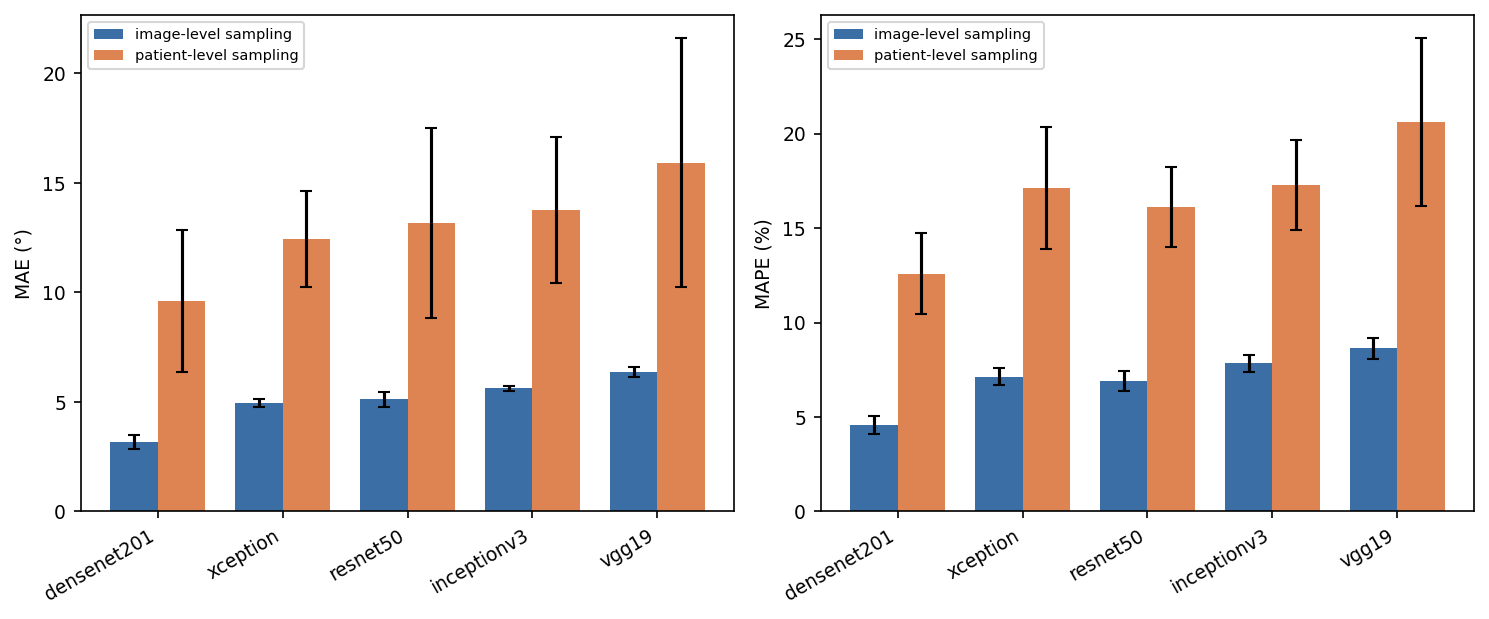
\includegraphics[width=0.92\linewidth]{figures/figure_protocol_comparison.png}
  \caption{Sampling-protocol sensitivity of the \emph{frozen} backbones with untuned grid-pooling heads (distinct from the Optuna-tuned estimator of Table~\ref{tab:dual_protocol}): per-backbone MAE (left) and MAPE (right) under image-level versus patient-level sampling. Both protocols are reported as five-fold cross-validation means with $\pm$1 standard-deviation whiskers. The cross-subject (patient-level) protocol is the harder regime, scoring generalization to unseen anatomy rather than across the augmented-image population, so every backbone shows a larger and more variable error there.}
  \label{fig:protocol_gap}
\end{figure}

\paragraph{Comparison to EMBC~2019.} The best single model of the original study reports $\approx\!\SI{2.87}{\degree}$ MAE / \SI{4.03}{\percent} MAPE under image-level sampling~\citep{Patil2019}. This work recovers that error band with a single tuned DenseNet201 (\SI{3.00}{\degree} MAE / \SI{4.03}{\percent} MAPE) and improves on it with the tuned stacked ensemble (\SI{1.96}{\degree} MAE / \SI{2.79}{\percent} MAPE, $R^2=0.995$), while additionally reporting the previously unmeasured patient-level number. The MAPE figures coincide at \SI{4.03}{\percent}; this is a numerical coincidence of two independently computed quantities, not a fitted match, and the MAE differs ($\SI{3.00}{\degree}$ here versus $\SI{2.87}{\degree}$ originally).

\subsection{Architecture bake-off: newer is not better}
\label{subsec:bakeoff}

A natural way to improve the patient-level estimator is to reach for a stronger or more recent backbone. We run an architecture bake-off under patient-level five-fold cross-validation, holding the grid-pooling head and training budget fixed and varying only the frozen encoder across classic ImageNet networks and the modern ConvNeXt~\citep{Liu2022} and EfficientNet / EfficientNetV2~\citep{Tan2019} families. Fig.~\ref{fig:bakeoff} summarizes the comparison.

No newer or larger backbone improves on DenseNet201. On the same era-2019 extraction that produced the modern bars, frozen DenseNet201 scores \SI{14.13}{\percent} ($\pm$\SI{2.19}{\percent}) MAPE, ahead of the best modern backbone, ConvNeXt-Base, at \SI{15.65}{\percent} ($\pm$\SI{1.75}{\percent}). These one-sigma bands overlap, so the margin is a consistent ordering across folds rather than a separation we can call significant; we report it as the matched comparison, not as a decisive gap. ConvNeXt-Tiny follows at \SI{16.07}{\percent}, and the EfficientNet / EfficientNetV2 B0--B3 variants trail from \SI{17}{\percent} to \SI{21.25}{\percent}. In its own fresh replication-era extraction DenseNet201 is lower still, \SI{12.59}{\percent}, but we lead with the matched number so the comparison is like-for-like.

The remaining classic backbones were extracted in the replication-era pipeline (ResNet50 \SI{16.12}{\percent}, Xception \SI{17.11}{\percent}, InceptionV3 \SI{17.29}{\percent}, VGG19 \SI{20.60}{\percent}), so they cannot be ranked against ConvNeXt strictly like-for-like, and we do not claim a firm classic-versus-ConvNeXt ordering among the non-DenseNet networks. Only DenseNet201 has a number on both extraction pipelines; the rest of the ranking is confounded by extraction era and should be read with that caveat. What is robust to extraction era is the narrow claim we make: on \num{84} base images of one narrow domain, with frozen features and a fixed head, no backbone newer or larger than the 2017 DenseNet201 beat it. We do not attribute this to a capacity ceiling, since we have not measured representation quality across encoders; the observation is bounded by this dataset and this protocol. DenseNet201 is the replication winner, the best frozen result here, and the strongest after tuning, so we carry it forward. This motivates the complementary strategy of the previous subsection: rather than change the backbone, tune the head and ensemble.

\begin{figure}[htbp]
  \centering
  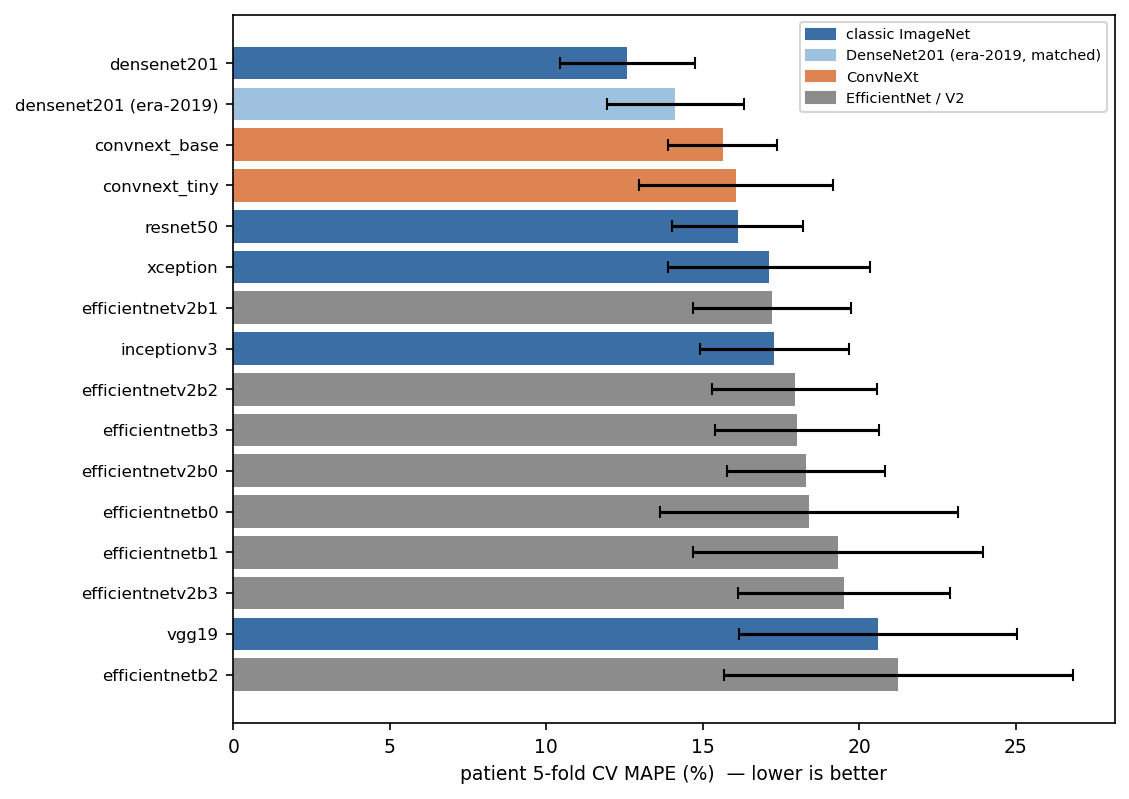
\includegraphics[width=0.78\linewidth]{figures/figure_architecture_bakeoff.png}
  \caption{Architecture bake-off under patient-level five-fold cross-validation (lower is better; bars are fold mean, whiskers $\pm$ one fold standard deviation; colour denotes the backbone family). All encoders are frozen with the identical grid-pooling head. A frozen DenseNet201 is the single best backbone, ahead of every modern ConvNeXt and EfficientNet / EfficientNetV2 variant; ConvNeXt is competitive with the other classic networks, so the result is that no newer or larger encoder improved on the 2017 DenseNet201 on this small, out-of-domain task, not that classic architectures win as a family. The five classic bars are the replication-era frozen extraction (\texttt{cmp\_*} rows); the ConvNeXt/EfficientNet bars are the era-2019 extraction (\texttt{f\_*}/\texttt{e2\_*} rows). The ordering is robust to this: even DenseNet201's era-2019 number (\SI{14.1}{\percent}) leads ConvNeXt-Base (\SI{15.7}{\percent}).}
  \label{fig:bakeoff}
\end{figure}

\subsection{Methods progression under patient-level sampling}
\label{subsec:progression}

Table~\ref{tab:methods_progression} traces how the patient-level estimator is built from frozen DenseNet201, with every step under the same patient five-fold cross-validation. The orientation-preserving grid-pooling head cuts the global-average-pooling baseline from \SI{18.70}{\percent} ($\pm$\SI{3.24}{\percent}) to \SI{12.59}{\percent} ($\pm$\SI{2.15}{\percent}) MAPE. Tuning that head with the Optuna TPE sampler~\citep{Akiba2019,Bergstra2011} brings it to \SI{10.80}{\percent} ($\pm$\SI{2.59}{\percent}), and Fig.~\ref{fig:tuning} shows the corresponding optimization history. The largest single gain comes from ensembling: combining the five tuned, patient-disjoint fold models and reading out their OOF predictions, a simple mean reaches \SI{9.89}{\percent} MAPE and a stacked combiner~\citep{Wolpert1992} reaches \SI{8.53}{\percent}, less than half the GAP baseline, entirely within the patient-level protocol.

Every row is measured under the same patient five-fold cross-validation, so the steps are directly comparable. The clinical-grade evaluation of the patient-level tuned ensemble is reported in Sec.~\ref{sec:evaluation}: conformal prediction intervals~\citep{Vovk2005,Lei2018}, Bland--Altman agreement~\citep{BlandAltman1986} against the single reference reading, test-time augmentation, and Grad-CAM~\citep{Selvaraju2017} attribution.

% AUTO-GENERATED by scripts/gen_paper_tables.py from results/ — DO NOT EDIT.
% Re-run: pixi run python scripts/gen_paper_tables.py
\begin{table}[htbp]
  \centering
  \caption{Methods progression for frozen DenseNet201 under the patient-level five-fold protocol (MAPE, \%): the global-average-pooling (GAP) baseline, the orientation-preserving grid-pooling head, Optuna tuning of that head, and the five-model out-of-fold ensemble. The single-model rows are per-fold CV means; the ensemble rows are computed on the pooled out-of-fold predictions (so no per-fold std is defined, ``--''). Aggregated the same pooled-OOF way, the tuned single DenseNet201 is \SI{10.14}{\percent} MAPE, so the genuine ensembling gain is \SIrange{10.14}{8.53}{\percent}; either way the ensemble breaks \SI{10}{\percent} on the cross-patient regime.}
  \label{tab:methods_progression}
  \begin{tabular}{lrrl}
    \toprule
    Method & MAPE (\%) & $\pm$std & Protocol \\
    \midrule
    DenseNet201, GAP head & 18.70 & $\pm$3.24 & patient 5-fold CV \\
    DenseNet201, grid pooling (frozen) & 12.59 & $\pm$2.15 & patient 5-fold CV \\
    DenseNet201, grid + Optuna-tuned & 10.80 & $\pm$2.59 & patient 5-fold CV \\
    \midrule
    Tuned 5-model ensemble (OOF mean) & 9.89 & -- & patient 5-fold OOF \\
    \textbf{Tuned 5-model ensemble (stacked)} & \textbf{8.53} & -- & patient 5-fold OOF \\
    \bottomrule
  \end{tabular}
\end{table}


\begin{figure}[htbp]
  \centering
  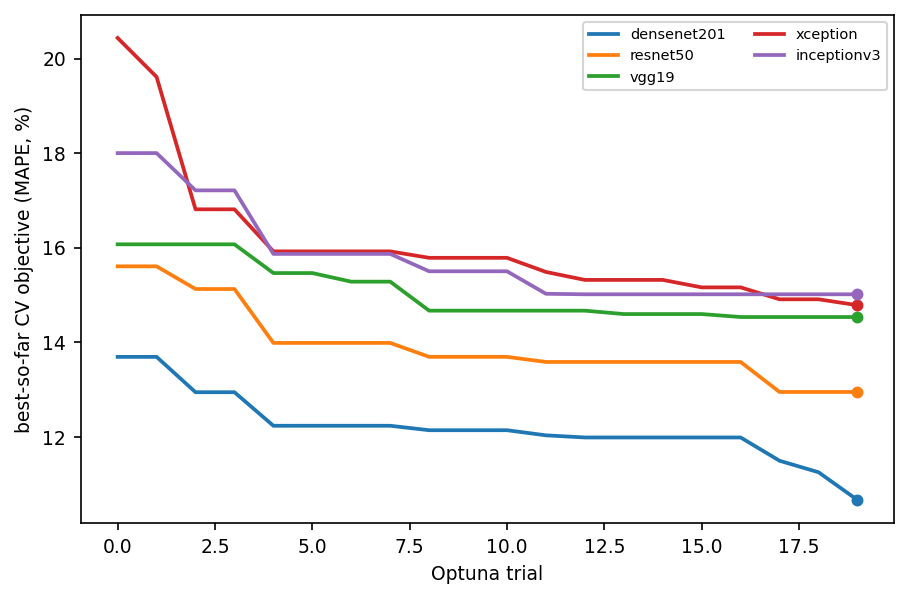
\includegraphics[width=0.62\linewidth]{figures/figure_tuning_history.png}
  \caption{Optuna TPE optimization history (best-so-far cross-validation objective vs trial) for each backbone's grid-pooling head and training hyperparameters under patient-level five-fold cross-validation. For DenseNet201 the best trial reaches a \SI{10.67}{\percent} search objective; the selected configuration, re-evaluated, scores \SI{10.80}{\percent} per-fold (Table~\ref{tab:methods_progression}), before ensembling.}
  \label{fig:tuning}
\end{figure}
